%!TEX program = xelatex


\documentclass[9pt,twocolumn,twoside]{pnas-new}
	% Use the lineno option to display guide line numbers if required.
	% Note that the use of elements such as single-column equations
	% may affect the guide line number alignment. 

	\templatetype{pnasresearcharticle} % Choose template 
	% {pnasresearcharticle} = Template for a two-column research article
	% {pnasmathematics} = Template for a one-column mathematics article
	% {pnasinvited} = Template for a PNAS invited submission

	\usepackage{csvsimple}
	% \usepackage{pc_writeup}
	\usepackage{pc_math}
	\usepackage[colorinlistoftodos]{todonotes}
	\usepackage{csquotes}

	% \usepackage{subcaption}
	% \usepackage{csquotes}

	\title{Diversity, Segregation, and Information in Cities}

	% Use letters for affiliations, numbers to show equal authorship (if applicable) and to indicate the corresponding author
	\author[a,b,1]{Philip Chodrow}

	\affil[a]{Human Mobility and Networks Laboratory, Massachusetts Institute of Technology, Cambridge, MA 02139}
	\affil[b]{Operations Research Center, Massachusetts Institute of Technology, Cambridge, MA 02139}

	% Please give the surname of the lead author for the running footer
	\leadauthor{Chodrow} 

	% Please add here a significance statement to explain the relevance of your work
	\significancestatement{Authors must submit a 120-word maximum statement about the significance of their research paper written at a level understandable to an undergraduate educated scientist outside their field of speciality. The primary goal of the Significance Statement is to explain the relevance of the work in broad context to a broad readership. The Significance Statement appears in the paper itself and is required for all research papers.}

	% Please include corresponding author, author contribution and author declaration information
	% \authorcontributions{Please provide details of author contributions here.}
	\authordeclaration{The author declares no competing interest.}
	% \equalauthors{\textsuperscript{1}A.O.(Author One) and A.T. (Author Two) contributed equally to this work (remove if not applicable).}
	\correspondingauthor{\textsuperscript{1}To whom correspondence should be addressed. E-mail: pchodrow@gmail.com}

	% Keywords are not mandatory, but authors are strongly encouraged to provide them. If provided, please include two to five keywords, separated by the pipe symbol, e.g:
	\keywords{Information Theory $|$ Diversity and Segregation $|$ Urban Theory} 

	\begin{abstract}
	Please provide an abstract of no more than 250 words in a single paragraph. Abstracts should explain to the general reader the major contributions of the article. References in the abstract must be cited in full within the abstract itself and cited in the text.
	\end{abstract}

	\dates{This manuscript was compiled on \today}
	\doi{\url{www.pnas.org/cgi/doi/10.1073/pnas.XXXXXXXXXX}}

% ----------------------------------------------------------------------------
% ----------------------------------------------------------------------------
% ----------------------------------------------------------------------------


\begin{document}

% Optional adjustment to line up main text (after abstract) of first page with line numbers, when using both lineno and twocolumn options.
% You should only change this length when you've finalised the article contents.
\verticaladjustment{-2pt}

\maketitle
\thispagestyle{firststyle}
\ifthenelse{\boolean{shortarticle}}{\ifthenelse{\boolean{singlecolumn}}{\abscontentformatted}{\abscontent}}{}

% If your first paragraph (i.e. with the \dropcap) contains a list environment (quote, quotation, theorem, definition, enumerate, itemize...), the line after the list may have some extra indentation. If this is the case, add \parshape=0 to the end of the list environment.
\dropcap{I}nformation theory...blah blah blah. 


\section*{Results}
	We model a city as a set of individuals distributed over a continuous spatial region $R$. 
	Each individual can belong to one of a set $\mathcal{Y}$ of racial groups, such as $\mathcal{Y} = \{\text{Asian}, \text{ Black}, \text{ Hispanic}, \text{ Other}, \text{ White}\}$. 
	The cross-tabulation of individuals and groups defines a probability $p(X,Y)$ that a randomly chosen individual from the city will live at location $X \in R$ and belong to group $Y$. 
	The population density at $x$ is $p(x) = \sum_{y \in \mathcal{Y}} p(x,y)$. 
	The global proportion of residents belonging to group $y$ is $p(y) = \int_R p(x,y)\; dx$. 
	The proportion of residents at $x$ belonging to group $y$ is $p(y|x) = p(x,y) / p(x)$. 
	To compare distributions to one another we use the Kullback-Leibler divergence 
	\begin{equation}
		D[q(A)\|r(A)] = \sum_{a \in \mathcal{A}} q(a) \log \frac{q(a)}{r(a)}\;.
	\end{equation}
	The divergence $D$ measures dissimilarity between distributions: it is zero if and only if $q = r$, and grows larger when $q$ and $r$ assign greater probability to different events. 

	

\subsection*{Entropy and Global Diversity}
	\emph{Global} measures of the city depend only on $p(Y)$, the global composition of racial groups. 
	The global Shannon entropy $H(Y)$ measures global diversity by comparing the global distribution $p(Y)$ to the uniform distribution $u(Y)$: 
	\begin{equation}
		H(Y) = -\sum_{y \in \mathcal{Y}}p(y) \log p(y) = \log \abs{\mathcal{Y}} - D[p(Y)\|u(Y)]\;.
	\end{equation}

	Local-to-global measures depend on comparisons between properties encoded by the local compositions $p(y|x)$ and the global composition $p(y)$. 

	Local measures depend only on comparisons between local compositions $p(y|x)$ and other nearby local compositions, without reference to the global composition $p(y)$. 
\begin{figure}%[tbhp]
		\centering % need to center this
		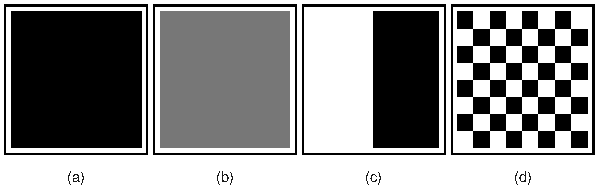
\includegraphics[width=\linewidth]{figs/checkerboard.pdf}
		\begin{tabular}{l | c c c} 
		City & $H(Y)$ & $I(X,Y)$ & $J(X,Y)$ \\
		\hline
		(a) & $0$        & $0$        & $0$\\
		(b) & $\log 2$ & $0$        & $0$\\
		(c) & $\log 2$ & $\log 2$ & $\frac{1}{7} \log 2$\\
		(d) & $\log 2$ & $\log 2$ & $\log 2$
		\end{tabular}
		\caption{
			\todo[inline=true]{Illustrate computation of $J$ on this fig?}
			Schematic cities illustrating three dimensions of segregation. 
			City (a) lacks global diversity, while cities (b)-(d) are maximally globally diverse. 
			City (b) is perfectly spatially even, whereas cities (c) and (d) are maximally uneven. 
			City (d) has higher spatial exposure than city (c) due to more contact points between racially distinct neighborhoods.
		} \label{fig:checkerboard}
	\end{figure}
\subsection*{Mutual Information and Spatial Evenness}
	Local-to-global measures depend on comparisons between properties encoded by the local compositions $p(Y|x)$ and the global composition $p(Y)$. 
	When each of the compositions $p(Y|x)$ is the same as $p(Y)$, the city is perfectly spatially even -- every racial group is represented at each location in proportion to their presence in the city overall. 
	When the local compositions $p(Y|x)$ differ from $p(Y)$, the city is spatially uneven. 
	We can measure spatial evenness as the average difference between local and global compositions: 
	\begin{equation}
		I(X,Y) = \E_X[D[p(Y|X)\|p(Y)]\;.
	\end{equation}
	The operator $\E_X$ denotes average or expectation with respect to the probability distribution of $X$. 
	$I(X,Y)$ is the \emph{mutual information}, a fixture of information theory. \cite{Bettencourt2015} 


	When all groups are evenly distributed, such as in Figure \ref{fig:checkerboard}(b), each location has the same composition as the global composition, and $I(X,Y) = 0$. 
	On the other hand, $I(X,Y)$ achieves its maximum value of $\log \abs{\mathcal{Y}}$ when every location is monogroup, such as in Figure \ref{fig:checkerboard}(c). 

\subsection*{Local Information and Spatial Complexity}
	
	Global and local-global measures can illuminate important high-level urban structure, but miss an important class of phenomena. 
	The model two-race cities (c) and (d) in Figure \ref{fig:checkerboard} each have the same values of $H(Y)$ and $I(X,Y)$. 
	City (c), however, has a single dividing line of racial separation, while city (d) has smaller pockets of racial distinctiveness. 
	In sociology or urban planning, this may be the difference between metastasized segregation and healthy variation. 
	The difference is intrinsically local, defined in terms of relations between local compositions $p(Y|X)$ and nearby other local compositions. 

	To measure local variation, imagine segmenting the city into a grid of small neighborhoods. 
	The \emph{local mutual information} in the neighborhood $B$ is the mutual information between $X$ and $Y$, restricted to $B$:
	\begin{equation*}
		I(X,Y | X \in B) = \E_{X|X \in B}[D[p(Y|X,X\in B)\|p(Y|X\in B)]\;.
	\end{equation*}
	The \emph{mean local information} measures the average local variation in group composition across the entire city:  
	\begin{equation}
		J(X,Y) = \E_B[I(X,Y|X \in B)]\;.
	\end{equation}
	If we regard the data as a discretization of a smooth probability field, then it is possible to show using arguments from information geometry \cite{Amari2000} that the local information in a neighborhood $B$ of radius $r$ is an approximation of the Fisher information $\mathcal{J}$:
	\begin{equation}
		I(X,Y|X \in B) \cong \frac{r^2}{4} \text{tr } \mathcal{J}_Y(x)\;, \label{eq:fisher_approx}
	\end{equation}
	where $[\mathcal{J}_Y(x)]_{ij} = \E_Y[-\partial_{x_i} \partial_{x_j} \log p(Y|x)]$ is the Fisher information matrix and $\text{tr } \mathcal{J}_Y(x)$ is the sum of its eigenvalues. 


	\begin{figure}
			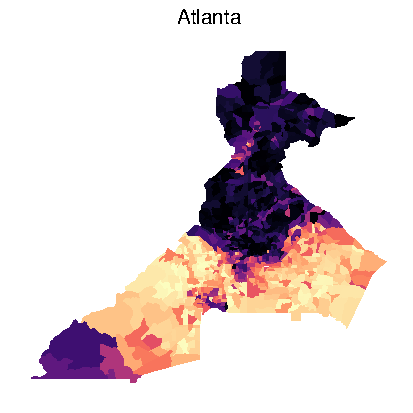
\includegraphics[width = .5\linewidth]{figs/Atlanta_percent_black.pdf}
			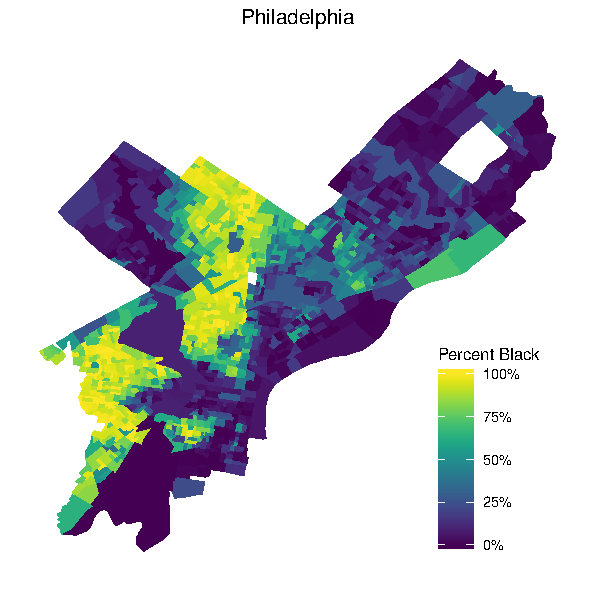
\includegraphics[width = .5\linewidth]{figs/Philadelphia_percent_black.pdf} \\
			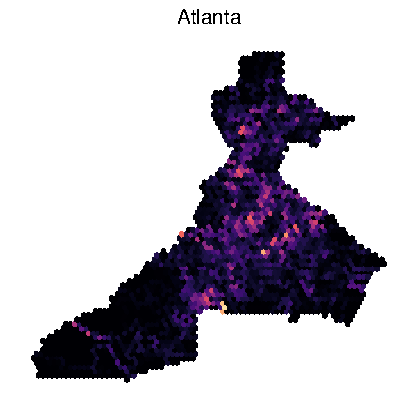
\includegraphics[width = .5\linewidth]{figs/Atlanta_grid.pdf} 
			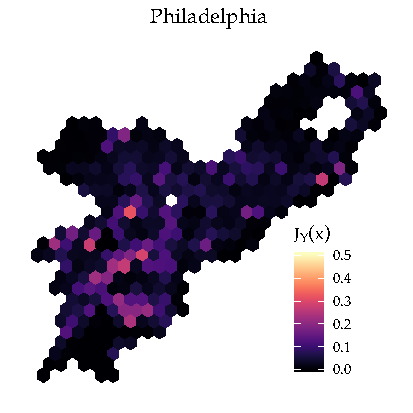
\includegraphics[width = .5\linewidth]{figs/Philadelphia_grid.pdf} \\

			\centering
			\begin{tabular}{l | c c c c}
				\bfseries City & Percent Black & $H(Y)$ & $I(X,Y)$ & $J(X,Y)$  \\\hline
				\csvreader[late after line=\\]{figs/comparative_summary.csv}{}
				{\csvcoli & \csvcolii & \csvcoliii & \csvcoliv & \csvcolv}
			\end{tabular}

			\caption{
				\todo[inline=true]{comment in here that it is possible to walk a km in Atlanta and basically see no change, not so in Philly}
				Spatial analysis of residential segregation in Atlanta and Philadelphia. 
				(\emph{Top}): Percentage of black residents. 
				(\emph{Middle}): Hexgrid of spatial resolution 1km imposed over each city. Within each hex $B$ we compute the local information local information $J_Y(B) = I(X,Y | X \in B)$. 
				(\emph{Bottom}): Numerical summary, including the three information measures.
			} \label{fig:Atlanta_philly}
	\end{figure}

\subsection*{Comparative Urban Analysis}
	
	We can view Atlanta and Philadelphia in broader context by comparing $I(X,Y)$ and $J(X,Y)$ across a range of American cities in Figure \ref{fig:mutual_fisher}. 
	For each city, we computed $J(X,Y)$ using a 1km hexgrid and the racial categories $\mathcal{Y} = \{\text{Asian}, \text{ Black}, \text{ Hispanic}, \text{ Other}, \text{ White}\}$. 
	The mutual information and local information sort cities into three primary classes. 
	Those toward the bottom left have low $I(X,Y)$ and therefore display relatively little spatial variation. 
	Cities become more unevenly distributed as we move rightward. 
	Those toward the bottom right, such as Atlanta and Detroit, are both highly uneven and have little local variation. 
	These cities are highly segregated, with large, starkly separated monoracial regions. 
	In contrast, cities toward the top right like Philadelphia and New York are more complex patchworks of smaller, ethnically distinct subregions.  

	\begin{figure}
		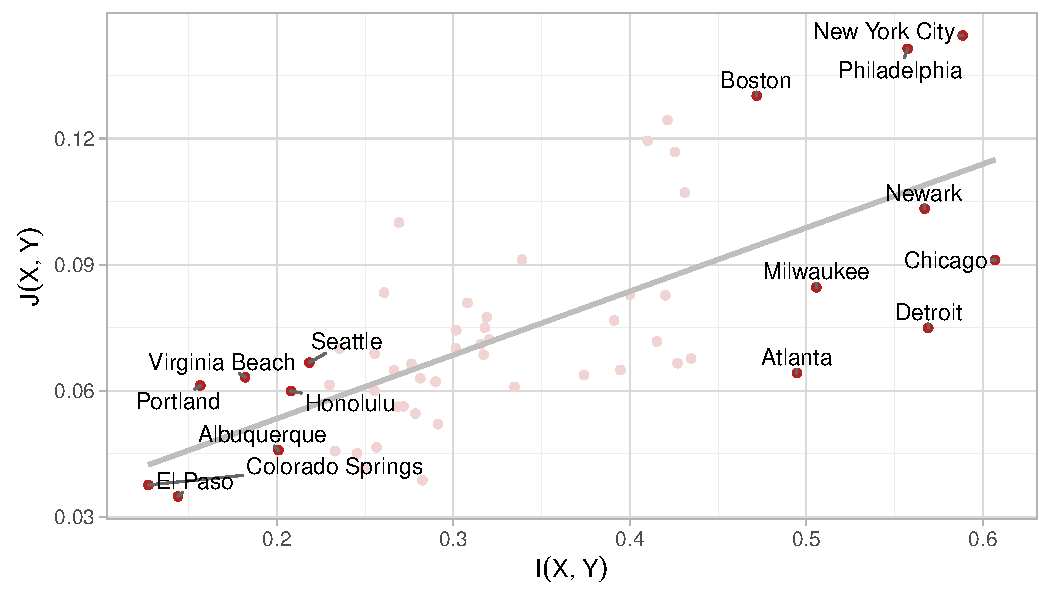
\includegraphics[width=\linewidth]{figs/mutual_fisher.pdf}
		\caption{
			Comparative global segregation measures in major U.S. cities, measured using racial categories $\mathcal{Y} = \{\text{Asian}, \text{ Black}, \text{ Hispanic}, \text{ Other}, \text{ White}\}$. 
			We used a hexgrid of spatial resolution $r = 1$km for the computation of $J(X,Y)$.
		} \label{fig:mutual_fisher}
	\end{figure}

\subsection*{Identifying Sociospatial Structure} 
	The measures $H(Y)$, $I(X,Y)$, and $J(X,Y)$ quantify the presence of global, local-global, and purely local sociospatial structure. We can also use information methods to identify and visualize that structure directly. While approaches exist to this problem,\footnote{For three, see \cite{Logan2011}} these approaches tend to conceptualize this structure in terms of monoracial subregions. In practice, however, there may be coherent biracial or multiracial patterns in space. Fortunately, it is possible to motivate a structure-finding algorithm for identifying high-level demographic trends without restriction to monoracial regions. 

	\begin{figure}

		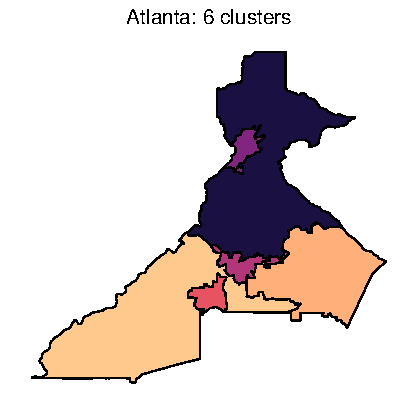
\includegraphics[width = .5\linewidth]{figs/Atlanta_clusters_binary_6.pdf} 
		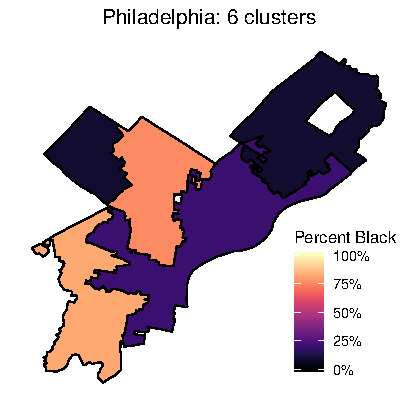
\includegraphics[width = .5\linewidth]{figs/Philadelphia_clusters_binary_6.pdf} \\
		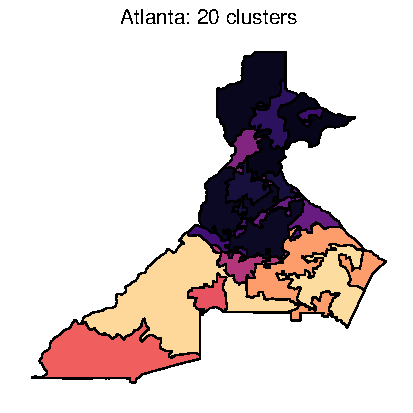
\includegraphics[width = .5\linewidth]{figs/Atlanta_clusters_binary_20.pdf}
		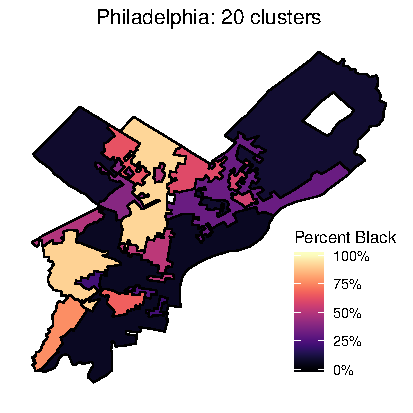
\includegraphics[width = .5\linewidth]{figs/Philadelphia_clusters_binary_20.pdf} \\
		
		\centering
		\begin{tabular}{l | c c c}
			\bfseries City  & $I(C_6, Y)$ & $I(C_{20},Y)$ & $I(X,Y)$ \\\hline
			\csvreader[late after line=\\]{figs/clustering_summary.csv}{}
			{\csvcoli & \csvcoliii & \csvcoliv & \csvcolii}
		\end{tabular}
		\caption{
			Example clusterings in Atlanta and Philadelphia using \eqref{eq:cluster_opt}, using $6$ and $20$ clusters. 
			The table below summarizes the between-groups mutual information captured by each cluster and compares it to the mutual information in the unaggregated blockgroup level data.
		} \label{fig:clusterings}

	\end{figure}
	Let $C$ be a random variable with the property that $H(C|X) = 0$; i.e. $X$ completely determines $C$. We can think of $C$ as group labels for the spatial locations $X$. Then, the chain rule of information\footnote{See \cite{Cover1991}} implies that 
	\begin{equation}
		I(X,Y) = \underbrace{I(C,Y)}_{\text{between-group}} + \underbrace{I(X,Y|C)}_{\text{within-group}}. \label{eq:chain_rule}
	\end{equation}

	Equation \eqref{eq:chain_rule} motivates a natural algorithm for identifying sociospatial structure. The core idea is that a clustering $C$ is ``good'' when it captures most of the intrinsic information in the system in the between-groups term $I(C,Y)$. Mathematically, we therefore wish to maximize $I(C,Y)$ subject to a fixed number of clusters, an approach popularized by \cite{Dhillon2003,Banerjee2005}. In full generality, this is a challenging discrete optimization problem that may not be computationally tractable. Additionally, for interpretability, we need to apply a spatial constraint: locales should be clustered together only when they are adjacent in space. To handle these two problems, we use a greedy algorithm based on agglomerative clustering. At stage of the algorithm, we consider the problem of choosing a pair of locales $\{i*, j*\}$ to aggregate together. A good choice of locales leads to minimal information loss, which we may quantify as follows. The mutual information over the full complement $\mathcal{K}$ of locales may be written: 
	\begin{align*}
	 	I(X,Y) &= \sum_{k \in \mathcal{K}} p(X = k) D[p(Y|X = k\|p(Y)] 
	\end{align*} 
	The contribution of locale $k$ to this sum is 
	\begin{align*}
		I_{k}(X,Y) &= p(X = k)D[p(Y|X = k)\|p(Y)]. 
	\end{align*}
	If we replace $i$ and $j$ with an aggregated locale $i\cup j$, the aggregated locale's contribution to the mutual information is 
	\begin{align*}
		I_{i\cup j}(X,Y) = p(X \in \{i,j\}) D[p(Y|X \in \{i,j\}) \| p(Y)]\;.
	\end{align*}
	The loss associated with aggregating $i$ and $j$ is the difference between their individual contributions and the aggregated contribution of $i\cup j$:
	\begin{align*}
		d(i,j) = I_{i}(X,Y) + I_{j}(X,Y) - I_{i \cup j}(X,Y).  
	\end{align*}
	The function $d$ may be regarded as a similarity measure. It satisfies $d(i,j) = 0$ if and only if $p(Y|X = i) = p(Y|X = j)$; i.e. the demographic profiles of locations $i$ and $j$ are identical. It is also symmetric in $i$ and $j$. It is not a true metric because it does not satisfy the triangle inequality. It can nevertheless be used to motivate a form of agglomerative hierarchical clustering, where at each phase of the algorithm we compute 
	\begin{equation}
		(i^*, j^*) = \argmin_{i \text{ neighbors } j} \; d(i,j)\; \label{eq:cluster_opt}
	\end{equation}
	and combine $i^*$ and $j^*$ into a single new region. We repeat this procedure until only $N$ regions remain. The optimization over $i$ and $j$ ensures that the groupings so defined approximate maximum between-group information partitions, and the constraint that $i$ must neighbor $j$ ensures that the structure so determined is spatially contiguous. Equation \eqref{eq:cluster_opt} thus defines \emph{spatially constrained, information-maximizing agglomerative clustering}. Since the algorithm is greedy, it possesses no guarantees of optimality, but in practice its performance leads to intuitive, demographically-coherent regions. 
	\todo[inline=true]{Should we state the algorithm in a figure?}
	
	\todo[inline=true]{Consider plotting the loss-curves in a readable way.}

	\begin{figure}
		\centering
			% \begin{subfigure}[b]{0.45\linewidth}
			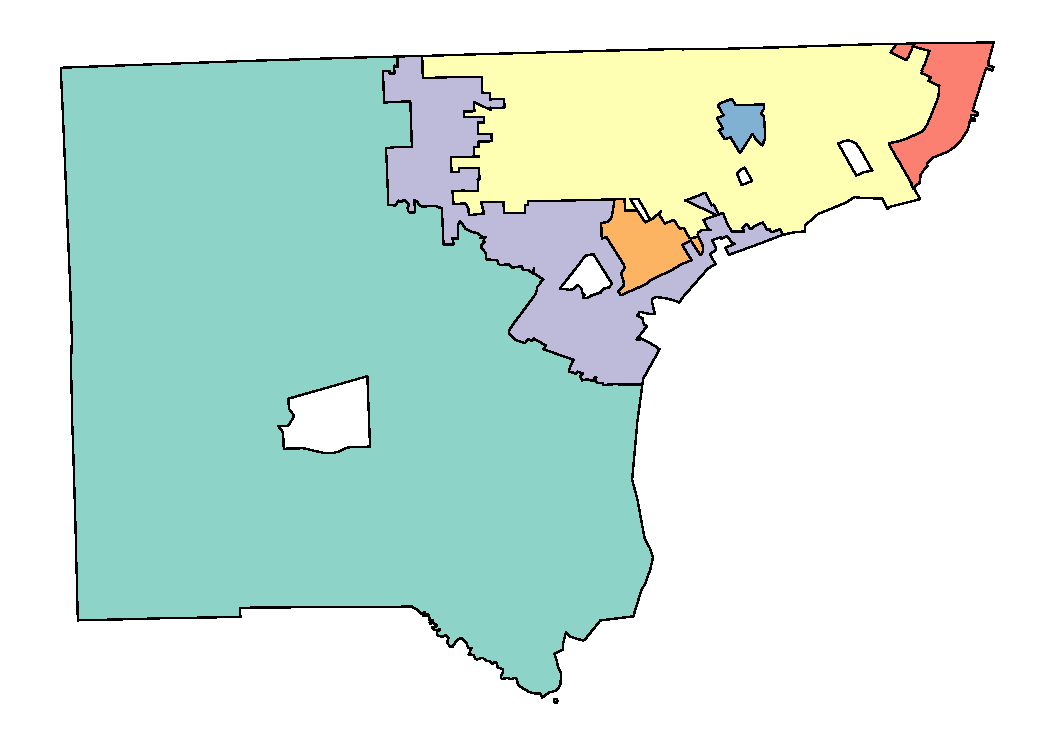
\includegraphics[width = .4\linewidth]{figs/example_cluster_map.pdf}
			% \caption{} \label{subfig:detroit_map}
			% \end{subfigure}
			% \begin{subfigure}[b]{0.45\linewidth}
			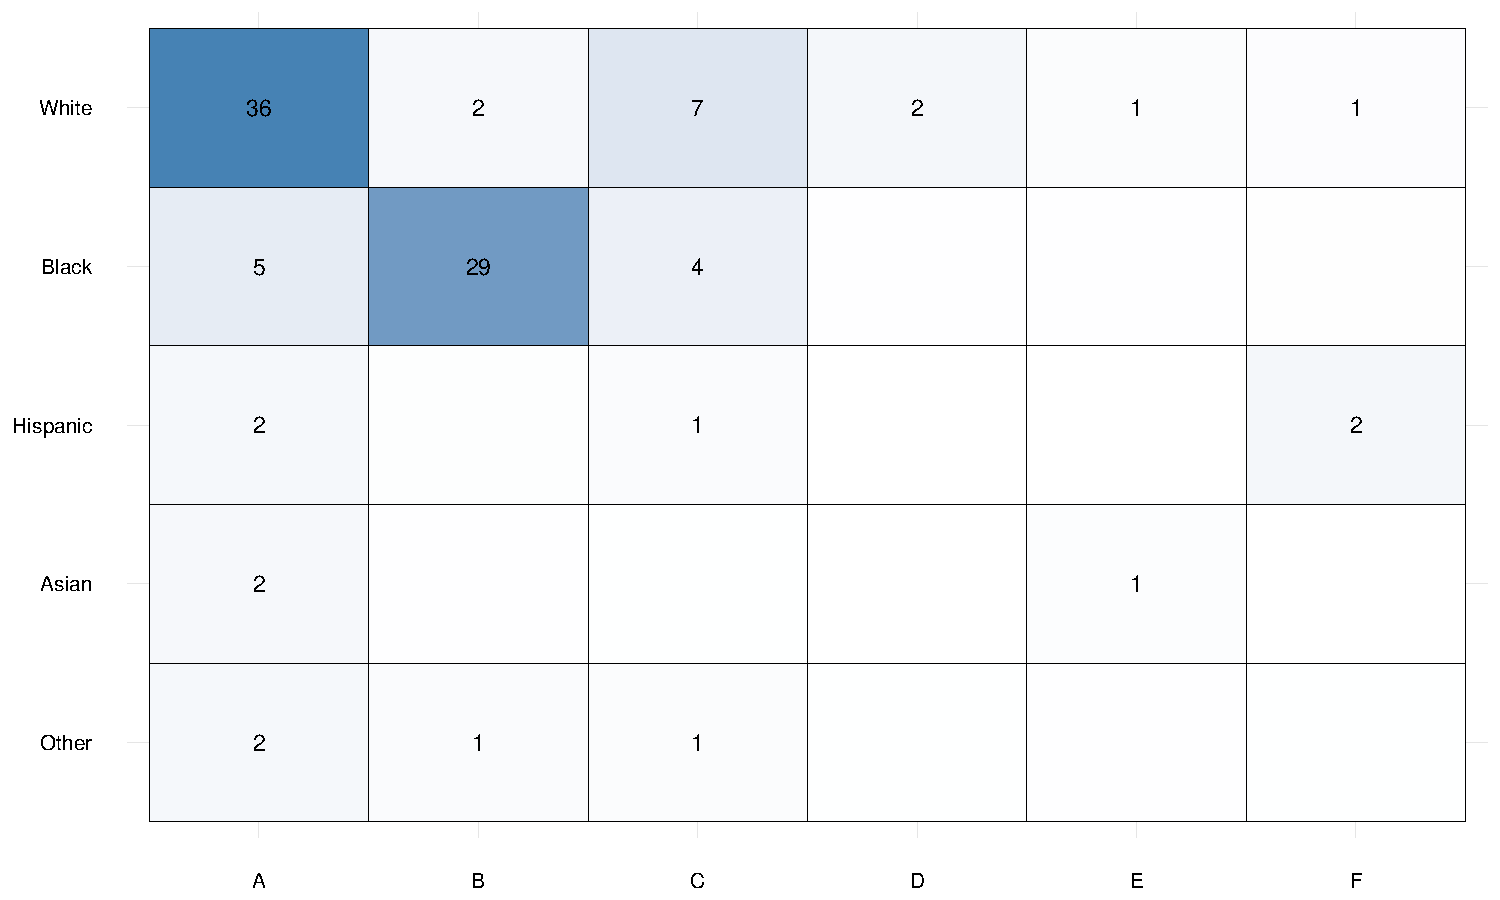
\includegraphics[width = .4\linewidth]{figs/example_clusters_detailed.pdf}
			% \caption{} \label{subfig:detroit_groups}
			% \end{subfigure}
			\caption{
				Multigroup sociospatial structure in Detroit. 
				\emph{(Left)}: Map of six clusters. 
				\emph{(Right)}: Joint distribution of demographics and clusters. 
				Shadings reflect population proportions within clusters. 
				Numerical labels give raw population proportions; for example, 29\% of the population is Black and resides in cluster B. 
				Detroit has $H(Y) = 1.12$, $I(X,Y) = 0.57$, and $J(X,Y) = 0.08$. 
				This clustering captures $I(C_6,Y) = 0.36$ nats of information.
			} \label{fig:detroit}
	\end{figure}

	This technique extends naturally to multi-group settings, though the visualization of results requires more subtlety. In Figure \ref{fig:detroit}, we conduct an illustrative analysis of multigroup segregation segregation in Detroit and the surrounding Wayne County. The prominent clusters A and B reflect the primary white/black division in the city, with A representing the white suburbs and B the denser black inner city. Cluster C is interpretable as a transitional area between these two populations, with both white and black residents represented. Cluster D coincides with the historically distinct, predominantly white town of Grosse Pointe. Cluster E coincides with the city of Hamtramck, whose history has been shaped by high levels of immigration from Europe and Asia. Finally, Cluster F coincides with the Hispanic neighborhood Mexicantown. 

	Aside from simply highlighting geographic trends, this analysis also enables the quantitative study of traditional concerns in segregation studies, such as concentration. According to \cite{Massey1988}, ``\emph{concentration} refers to the degree of a group's agglomeration in urban space.'' The concept of concentration invites us to consider the composition and density of each cluster. For example, whites make up 70\% of ``their'' cluster A, while black residents make up 86\% of ``their'' cluster B. Cluster B is also more densely populated than Cluster A: it contains 34\% of Wayne County's population, but just 19\% of the analyzed geographic area, making it more than twice as dense as Cluster A. Thus, in and around Detroit, black neighborhoods tend to be both more racially homogeneous and more densely packed in urban space than white ones. We can also learn about pairwise group exposure. For example, from Figure  \ref{subfig:detroit_groups}, we observe that Asian residents tend to be found alongside white residents, but more rarely alongside black or Hispanic residents. Hispanic residents tend to group in Mexicantown and in predominantly white neighborhoods -- not black ones.

\subsection*{Evaluating Clusterings}
	As discussed, the mean local information $J(X,Y)$ can be viewed as a measure of the number and character of transitional areas between regions of differing demographic structure.  It is low in Atlanta because the city is dominated by one, large North-South boundary while it is higher in Philadelphia due to many points of contact between neighborhoods of differing composition. Sociospatial transitions are also precisely the ``fault lines'' along which we would expect the clustering algorithm \eqref{eq:cluster_opt} to split the city. It is therefore not a coincidence that Philadelphia both has a higher value of $J(X,Y)$ and requires a greater number of clusters to convey a similar amount of sociospatial information. 

	To quantify the relationship between the mean local information $J(X,Y)$ and the clustering method \eqref{eq:cluster_opt}, we must first quantify the performance of the latter. We can do this by considering the number of clusters necessary to convey a given fraction of overall mutual information. Consider the between-groups information $I(C_n,Y)$ plotted as a function of the number $n$ of clusters. The result is a curve reflecting how information scales at varying levels of aggregation. Figure \ref{fig:AUC} shows examples of these curves for Atlanta, Detroit, and Philadelphia, with $N$ plotted on a logarithmic scale. The area under the curve (AUC) serves a measure of how early information is ``captured'' by the clustering. When the AUC is high, small numbers of clusters suffice to capture most of the information; when it is low more complex clustering is necessary. The AUC can be computed explicitly via the formula 
	\begin{equation}
		AUC = \frac{1}{I(X,Y) \log N} \sum_{n=1}^N I(C_n, Y) \log \frac{n+1}{n}, \label{eq:AUC_formula}
	\end{equation}

	AUC is therefore an algorithmic measure of sociospatial complexity, which is high when there are few sociospatial boundaries and low when there are many. Previously, we also argued that the quantities $H(Y)$, $I(X,Y)$, and $J(X,Y)$ may be viewed as information measures of sociospatial complexity, and particularly that $J(X,Y)$ measures the presence of sociospatial boundaries. We should therefore expect that these two sets of measures are related. A simple way to test for the relationship is via linear least squares regression. We aim to approximate the AUC via the formula
		\begin{equation*}
			AUC \approx m_1H(Y) + m_2I(X,Y) + m_3J(X,Y) + b\;.
		\end{equation*}
	The results of this approximation are shown in Figure \ref{fig:regression}. Collectively, the three information measures suffice to explain an adjusted 75\% of the variation in the AUC, confirming that both the information measures and the algorithmic AUC measure the same underlying sociospatial structure. The coefficients are also instructive. The largest magnitude by far is the coefficient of $I(X,Y)$; all else equal, clustering is more effective when groups are distributed unevenly. The negative sign on the coefficient of the mean local information $J(X,Y)$ confirms our specific expectations from above; for fixed $I(X,Y)$ and $H(Y)$, a city with higher $J(X,Y)$ (more sociospatial complexity) is more difficult to model or simplify than one with lower $J(X,Y)$. 

	\begin{figure} 
			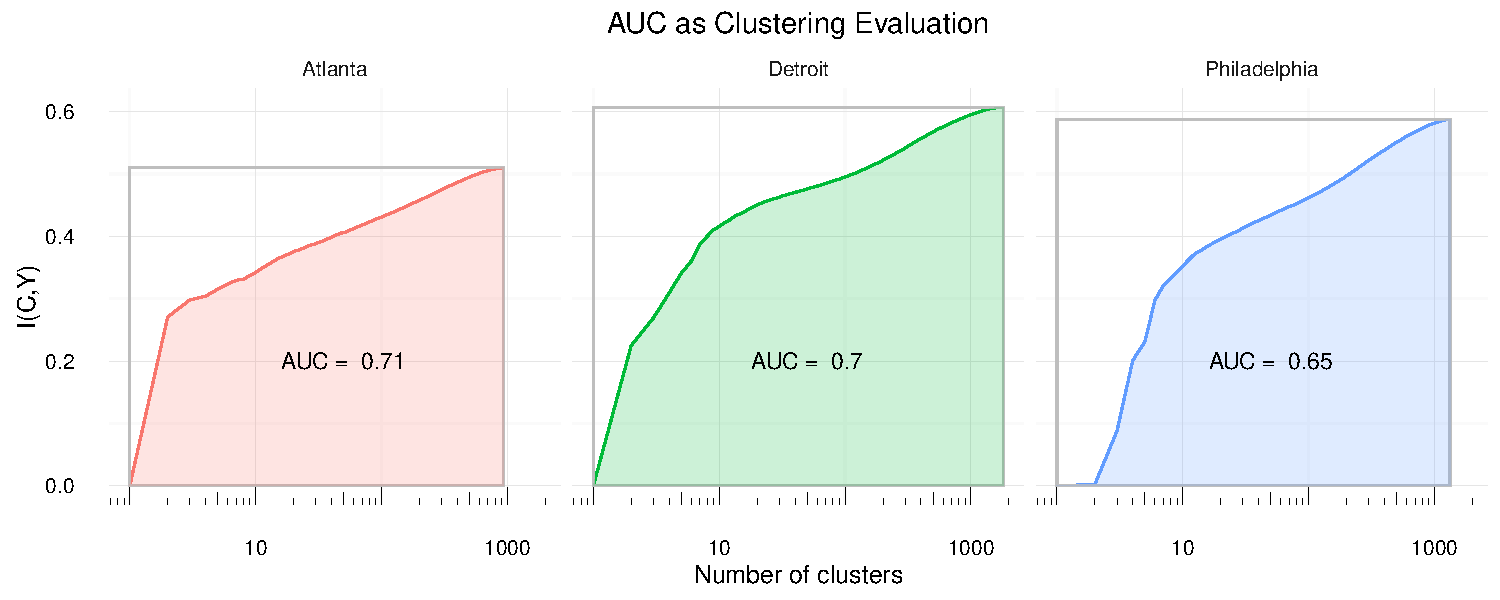
\includegraphics[width=\linewidth]{figs/AUC_illustration.pdf}
			\caption{
				Evaluation of clusterings using the area under the curve (AUC) for $\mathcal{Y} = \{\text{Black }, \text{Non-Black}\}$, computed according to the formula \eqref{eq:AUC_formula}. 
				The bounding rectangle for each city is shown in grey. 
				The AUC is the proportion of the rectangle contained in the shaded region. 
				The AUC for Philadelphia has been adjusted to account for the data set's two disconnected geographic components.
			} \label{fig:AUC}
	\end{figure}
	\begin{figure}
		\centering
		\input{figs/adjusted_regression.txt}
		\caption{
			Regression of the AUC computed by \eqref{eq:AUC_formula} on the information measures $H(Y)$, $I(X,Y)$, and $J(X,Y)$. 
			95\% confidence intervals for each of the determined coefficients are shown in parentheses. 
			The three information measures jointly explain an adjusted 75\% of the variation in the AUC. 
		}\label{fig:regression}
	\end{figure}

\section*{Discussion}
	
	\subsection*{Local Information as a Complexity Measure}
		The local information $J(X,Y)$ is a measure of spatial exposure contextualized by the mutual information. It can also be viewed as a measure of \emph{intrinsic sociospatial complexity}. Cities with high mean local information, such as Philadelphia, have more complex spatial structure than those with low mean local information such as Atlanta. Urban complexity has been a lively topic of interest at the intersection of physics and urban planning. Physically, the complexity of cities can be viewed as a rough measure of the complexity of theories needed to explain their structure and dynamics \cite{Bettencourt2015}. From a planning perspective, the complexity of land use was famously theorized by Jane Jacobs \cite{Jacobs1992} to be a driver of the health of neighborhoods. This theory has received preliminary empirical support \cite{DeNadai2016a}, with more tests no doubt to come. The local information can capture local variations in land use as well as demographics. We hope that this measure will serve as a useful tool for scholars of urban spatial complexity.  
	\subsection*{Local Information as a Complexity Measure}
		A major challenge for information theory in urban science is the development of principled dynamical models that can explain variations in observed information measures across cities \cite{Batty2014a}. One approach to this challenge is to observe how information changes over time at varying scales. On the timescale of decades, information measures may be used to analyze the evolution of the evolving sociospatial structure of cities. Information-maximizing agglomerative clustering could then be used to cluster coherent regions in time as well as space, enabling a view of shifting demographic boundaries.

		Another avenue of exploration is on the much shorter timescale of daily mobility. Many adults spend less than half of their waking hours at home \cite{BureauofLaborStati2014}, indicating that residential segregation is only a partial characterization of city-wide diversity. Fortunately, our ability to learn about daily patterns of human mobility is progressing at a rapid pace. Recent years have seen an enormous increase in the use of mobile devices, allowing the passive collection of digital traces. These traces can be processed, analyzed, and validated to derive insight into daily activity patterns \cite{Widhalm2015,Yang,Jiang2013,Jiang2012c}. By combining these traces with residential demographics, it is possible to estimate flows of different demographic groups throughout the city on a daily basis. 
	\subsection*{Spatial Preprocessing}
		The measures we have developed use their data (provided by the Census) as an unbiased approximation of the true distribution of racial groups across locations. This approach has two limitations. First, the demarcations of Census areal units are to some extent arbitrary: changing them would not change the underlying demographic phenomena, but may change the values of the mutual information or local information \cite{Openshaw1981}. Second, cities are anisotropic: two neighborhoods may be no more than 50 meters away, but if they are separated by a river, they may be functionally ``farther'' from each other than two other neighborhoods 500m apart. An approach to address both criticisms is to spatially preprocess the data using a smoothing kernel, as demonstrated in \cite{Roberto2015} for the case of the mutual information. Further experiments on the numerical impact of MAUP and anisotropy are called for in order to determine whether the benefit of preprocessing justifies the additional computational costs of this procedure.   


\matmethods{
		\subsection*{Data Access}
		All data used in this study are freely available from the U.S. Census. The \texttt{R} packages \texttt{acs} and \texttt{tigris} were used to programmatically download demographics and geographic shapefiles, respectively. All demographic data is from the Five-Year Estimates of the 2014 American Community Survey, Table B03002. 
		\subsection*{Software Repositories}
			We are pleased to make available two software repositories accompanying this analysis. Package \texttt{compx} for the \texttt{R} programming language implements computation of the information measures $H(Y)$, $I(X,Y)$, and $J(X,Y)$, as well as a method for information-theoretic clustering. Access \texttt{compx} at \texttt{https://github.com/PhilChodrow/compx}. 
			
			The analysis repository for this project includes data acquisition and processing; core computations; and figure generation. We hope that this repository will provide useful examples of how to use \texttt{compx} for others aiming to replicate and extend our results. Download the project files at \texttt{https://github.com/PhilChodrow/spatial\_complexity}. 
			  
		\subsection*{Delimiting Cities} 
		The delimiting of cities based on non-arbitrary population densities or natural boundaries is an area of active discussion in urban planning. For recent advances, see \cite{Rozenfeld2008,Rozenfeld2011}. W took a simple approach for the purposes of this study. For each city considered, we analyzed the region composed of all (and only those) counties in which some or all of the city's municipal boundaries lie. For example, our region corresponding to Atlanta consists of Fulton and Dekalb Counties, our region corresponding to Philadelphia consists of Philadelphia County, and the region corresponding to Detroit consists of Wayne County. For independent cities such as Baltimore and Washington D.C., the region of analysis consists simply of the municipal city boundaries. 
		\subsection*{Aggregation of Racial Categories} 
		The data provided by Table B03002 contains categories corresponding to two options for ethnicity (Hispanic or Latino, Not Hispanic or Latino) and nine corresponding to race, giving a total of 18 cross-tabulated categories. For the purposes of analysis, we aggregated these into just five categories, \{\text{Asian}, \text{Black}, \text{Hispanic}, \text{Other}, \text{White}\}. The correspondence used is given in the GitHub repository \texttt{PhilChodrow/spatial\_complexity} linked above, under \texttt{assumptions/race\_lookup.csv}. 
		\subsection*{Analysis and Visualization} 
		All analysis and visualization was conducted in the \texttt{R} statistical programming language. We used \cite{Bivand2014b,Bivand2014a,Bivand2014} for geographic analysis, and \cite{Wickham} for visualization.
}

\showmatmethods{} % Display the Materials and Methods section

\acknow{P.C. is grateful to Marta C. Gonz\'{a}lez for helpful discussion, and to MIT-Saudi Arabia...}

\showacknow{} % Display the acknowledgments section

% \pnasbreak splits and balances the columns before the references.
% Uncomment \pnasbreak to view the references in the PNAS-style
% If you see unexpected formatting errors, try commenting out \pnasbreak
% as it can run into problems with floats and footnotes on the final page.
% \pnasbreak

% \nocite{Bettencourt2013}

% Bibliography
\bibliography{/Users/phil/bibs/library.bib}

\end{document}